\begin{figure}[H]
    \centering
    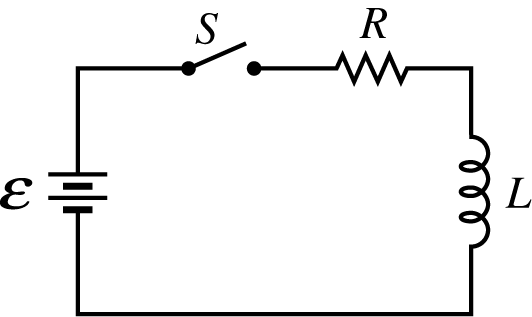
\includegraphics[scale=0.3]{images/img-005-007.png}
\end{figure}

% Multiple Choice Question 7
\begin{questions}\setcounter{question}{6}\question
Time $t$ is the time it takes the current of an $L R$ circuit with an inductor of inductance $L$ and a resistor of resistance $R$ to reach half of its maximum value. What is the new time if the original inductor is replaced with an inductor of inductance $2 L$ ?

\begin{oneparchoices}
\choice $4 t$
\choice $2 t$
\choice $t$
\choice $t / 2$
\choice $t / 4$
\end{oneparchoices}\end{questions}

